\documentclass[a4paper, 10pt, fleqn]{article}

\usepackage[utf8]{inputenc}
\usepackage[T1]{fontenc}
\usepackage{textcomp}
\usepackage{lmodern}
\usepackage[ngerman]{babel}
\usepackage{tocbibind}
\usepackage{enumerate}
\usepackage{xcolor}
\usepackage{pdfpages}
\usepackage{amsmath}
\usepackage{graphicx}
\usepackage{geometry}
\usepackage{scrpage2}
\usepackage{lastpage}
\usepackage[hyphens]{url}
\usepackage{hyperref}
\usepackage{listings}
\usepackage{float}
\restylefloat{figure}
\lstset{language=[ansi]C++}

\newcommand{\code}[1]{\texttt{#1}}

\renewcommand*{\listoffigures}{%
  \begingroup
  \tocchapter
  \tocfile{\listfigurename}{lof}
  \endgroup
}

\geometry{left=3cm, top=3cm, bottom=3cm, right=2cm}

\hypersetup{
    colorlinks,
    linkcolor=black,
    citecolor=black,
    urlcolor=black
}

\pagestyle{scrheadings}
\ihead{PREN2 Gruppe 39}\ohead{UART Interface Spec} 
\ifoot{\today} \ofoot{Seite \thepage\ von {\hypersetup{linkcolor=black}\pageref{LastPage}}}

% Einrücken zu Beginn von neuem Absatz unterdrücken
\setlength{\parindent}{0pt}

\begin{document}
% !TEX root = Dokumentation.tex
\begin{titlepage}   

\begin{center}
\textsc{\Large PREN Team 39}\\[0.5cm]

% Title
\newcommand{\HRule}{\rule{\linewidth}{0.5mm}}
\HRule \\[0.4cm]
{ \huge \bfseries GüselStar XXI}\\[0.4cm]
{ \LARGE \bfseries Gesamtkonzept}\\[0.4cm]
\HRule \\[1.5cm]

% Unterer Teil der Seite
{\large Horw, \today}

\begin{figure}[H]%Position festigen
\centering
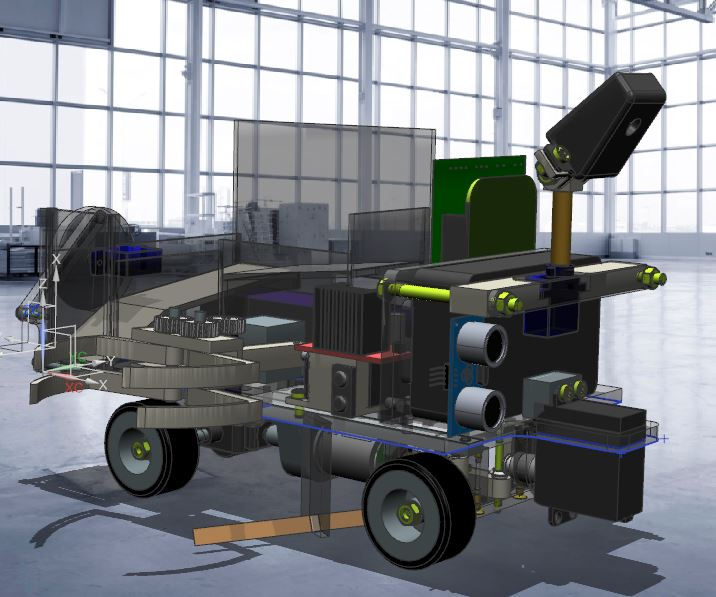
\includegraphics[width=0.7\textwidth]{03_Loesungskonzept/pictures/Tietelbild1.JPG}
\label{fig:activityRoute}
\end{figure}
% Author and supervisor
\begin{minipage}{0.4\textwidth}
\begin{flushleft} \large
\emph{Autoren:}\\
Patrizio Brantschen\\
Stefan Häfliger\\
Tobias Kreienbühl\\
Joël Meloni\\
Silvan Ritz\\
Lars Walther\\
\end{flushleft}
\end{minipage}
\hfill
\begin{minipage}{0.4\textwidth}
\begin{flushright} \large
\emph{Supervisor:} \\
Jürg Habegger
\end{flushright}
\end{minipage}
\large
\vfill
TA.BA\_PREN2.F1601 \\
Hochschule Luzern Technik \& Architektur

\end{center}

\end{titlepage}
\tableofcontents
\clearpage
\newpage
\section{Systemübersicht}
Aufgabe der UART Schnittstelle ist es, die Kommunikation zwischen Minicomputer und Mikrocontroller sicherzustellen. Dazu gehören folgende Aufgaben
\begin{itemize}
\item Austausch der Sensorwerte für die Regelkreise.
\item Definierte Kommandos um die Aktoren anzusteuern.
\end{itemize}
\section{Architektur und Designentscheide}
Um den Datenfluss einfach zu halten, werden Sensorwerte periodisch vom Freedom Board an das Raspberry Pi übertragen. Die Klasse \code{UARTReciever} ist entsprechend als Thread realisiert entschlüsselt den empfangenen String und schreibt den Wert auf entsprechende Member-Variabeln. Diese können über Funktionsgerechte Get-Methoden abgefragt werden.\\
Das Senden von Daten wird ebenfalls über Funktionsgerechte Send-Methoden von der Klasse \code{UARTSender} zur Verfügung gestellt. Entsprechend setzen diese Methoden die Ausgabestrings zusammen.
\section{Methodendefinitionen}
\subsection{UART-Methodenstrings}
\begin{tabular}{|l|l|l|l|l|} \hline
Aktion/Aktor         & Richtung     & String,[params]    & Übergabewert              & Bemerkungen \\\hline\hline
Ultraschall          & Frd$\to$Rasp & Ul,uint16          & distance cm               & periodisch all 0.3s \\\hline
Flexsensor1 und ev 2 & Frd$\to$Rasp & Fld1,uint8         & distance mm               & periodisch all 0.2s \\\hline
StatusAuf            & Rasp$\to$Frd & StA d,uint16       & distance mm               & \\
                     & Frd$\to$Rasp & StAf               &                           & Wenn  abgeschlossen \\\hline
StatusAb	             & Rasp$\to$Frd & StE d,uint16       & distance mm               & \\
                     & Frd$\to$Rasp & StEf               &                           & Wenn abgeschlossen\\\hline
DC Motor             & Rasp$\to$Frd & DCDr d,uint8,uint8 & mm pro sek.,modus         & Modi: hard/soft \\
                     & Frd$\to$Rasp & DCDr,uint8         & mm pro sek.               & wenn encoder say o \\\hline
Lenkungsservo        & Rasp$\to$Frd & LeS p,uint8        & abs Winkel (0=127)        & \\\hline
Kameraservo          & Rasp$\to$Frd & CamP p,uint8       & Kamera pos                & \\\hline
Debug Messages       & Frd$\to$Rasp & DBG,char[]         & Meldung                   & \\\hline
NochDa               & Frd$\to$Rasp & There              & Flag                      & periodisch all 0.5s \\
                     & Rasp$\to$Frd & Ja                 & Erhalten?                 & Wenn nein $\to$ DC stop \\\hline
Start                & Rasp$\to$Frd & StartFrd           &                           & Hochfahren und init \\
                     & Frd$\to$Rasp & Ready              &                           & \\\hline
Stop	                 & Rasp$\to$Frd & Stop               &                           & Programm beenden \\
	                 & Frd$\to$Rasp & Stop               &                           & Programm beendet \\ \hline
\end{tabular}
\subsection{Methodenübersicht \code{UARTReciever}}
\begin{itemize}
\item \code{int getFlexDistance(void)} Methode, die den Abstand des Flexsensors zurückgibt.
\item \code{int getEngineSpeed(void)} Methode, die des Antriebsmotors aktuelle Geschwindigkeit zurückgibt.
\item \code{int getUltraDist(void)} Methode liefert die kürzeste Distanz des Ultraschallsensors zurück.
\end{itemize}
\subsection{Methodenübersicht \code{UARTSender}}
\begin{itemize}
\item \code{bool sendStartCmd(void)} Methode, die das Freedom Board aktiviert und alle Aktoren in Ausgangsposition bringt. Rückgabe: \code{false}, wenn ein Übertragungsfehler aufgetreten ist, \code{true} sonst.
%
\item \code{bool sendStopCmd(void)} Methode, welche dem Freedom Board das Ende des Programms signalisiert.  Rückgabe: \code{false}, wenn ein Übertragungsfehler aufgetreten ist, \code{true} sonst.
%
\item \code{bool setCameraPos(CameraStatesE pos)} Methode dreht die Kamera auf die gewünschte Position. Übergabewerte: \code{CAM\_STRAIGHT} = gerade, \code{CAM\_CHECK\_STREET} für Rechtsvortritt, \code{CAM\_TURN\_RIGHT} = Rechtskurve und \code{CAM\_TURN\_LEFT} = Linkskurve. Rückgabe: \code{false}, wenn ein Übertragungsfehler aufgetreten ist, \code{true} sonst.
%
\item \code{bool setEngineSpeed(uint8\_t speed, EngineModesE mode = SOFT)} Methode setzt den Motor auf die gewünschte Geschwindigkeit, der Modus kann zwischen \code{SOFT} (default) und \code{HARD} gewählt werden. \code{HARD} = Notfall. Rückgabe: \code{false}, wenn ein Übertragungsfehler aufgetreten ist, \code{true} sonst.
%
\item \code{bool setContainerFound(uint16\_t distance)} Methode teilt dem Mikrocontroller mit, einen Container gefunden zu haben. Übergabeparameter: Abstand zum Container. Rückgabe: \code{false}, wenn ein Übertragungsfehler aufgetreten ist, \code{true} sonst.
%
\item \code{bool setTargetFieldFound(uint16\_t distance)}  Methode teilt dem Mikrocontroller mit, das Ziel gefunden zu haben. Übergabeparameter: Abstand zum Zielfeld. Rückgabe: \code{false}, wenn ein Übertragungsfehler aufgetreten ist, \code{true} sonst.
%
\item \code{bool setSteering(uint8\_t steeringAng)}  Methode teilt dem Mikrocontroller mit, das auf einen bestimmten Winkel gelenkt werden soll. 0 Grad = 127 aufgrund des unsigned Typen. Übergabeparameter: Winkel, auf den die Lenkung gestellt werden soll. Rückgabe: \code{false}, wenn ein Übertragungsfehler aufgetreten ist, \code{true} sonst.
%
\item \code{bool stillThereResponse(void)} Methode sendet ein Ja auf die Frage, ob die Verbindung noch steht.  Rückgabe: \code{false}, wenn ein Übertragungsfehler aufgetreten ist, \code{true} sonst.
\end{itemize}
\end{document}